\documentclass[aspectratio=169]{beamer}
\mode<presentation> {
\usetheme{default}
\usecolortheme{dolphin}
}
\usepackage{algorithm,algorithmic}
\usepackage{caption}
\usepackage{multirow}
\usepackage{threeparttable}
\usepackage{natbib}
\bibliographystyle{aer}
\usepackage{graphicx}
\usepackage{parskip}
\usepackage{float}
\usepackage{alphabeta}
\usepackage{multirow,array}
\usepackage{subfig}
\usepackage{amsmath}
\usepackage{amssymb}
\usepackage{mathabx}
\usepackage{caption}
\usepackage{pifont} 
\usepackage{booktabs,tabularx}
\newcolumntype{Y}{>{\raggedright\arraybackslash}X}

\usepackage{tikz}
\usetikzlibrary{arrows.meta,positioning,calc,fit,backgrounds,decorations.pathreplacing, shapes.geometric}
\graphicspath{{figures/}}

% TikZ Styles - Adjusted font sizes for clarity since bold is removed
\tikzset{
  >=Stealth,
  st/.style={circle,draw,inner sep=0pt,minimum size=6mm, fill=white}, 
  action/.style={circle,fill=black,inner sep=0pt,minimum size=2mm},
  tr/.style={-Stealth, line width=0.8pt},
  lbl/.style={font=\footnotesize},
  block/.style={rectangle, draw, fill=blue!10, rounded corners, minimum height=2em}
}

\newcommand{\E}{\mathbb{E}}
\newcommand{\R}{\mathbb{R}}
\newcommand{\1}{\mathbf{1}}
\DeclareMathOperator*{\argmax}{arg\,max}
\DeclareMathOperator*{\argmin}{arg\,min}
\setbeamertemplate{caption}[numbered]
\setbeamertemplate{navigation symbols}{}
\setbeamertemplate{footline}[frame number]

\title{Lecture 8: Simulation-Based Learning }

\author{Yasuyuki Sawada, Yaolang Zhong}
\institute{University of Tokyo\\
  \small \texttt{\href{mailto:yaolang.zhong@e.u-tokyo.ac.jp}{yaolang.zhong@e.u-tokyo.ac.jp}}}
\date{\today}

\begin{document}

\begin{frame}
\titlepage  
\end{frame}

%===================================================
% MOTIVATION AND CONTEXT
%===================================================

\begin{frame}{Recap: The Computational Challenge}
\small
\begin{itemize}
    \item Recall the Bellman Equation:
    \[
        V(s) = \max_{a} \left\{ r(s, a) + \beta \int V(s') P(ds' \mid s, a) \right\}
    \]
    \item So far, deterministic update:
        \begin{itemize}
            \item enumerate all states $s \in \mathcal{S}$ (use a fixed grid in the continuous case)
            \item update $V(s)$ by enumerating over all states $s' \in \mathcal{S}$ and integrating over $P$
            \item Lecture 7: introduce stochasticity by Monte Carlo integration (but still iterate over all $s$)
        \end{itemize}
    \item However: Enumerating all states $s$ means we want accurate $V(s)$ everywhere: the evaluation and update is costly, but the contrubution to gain in accuracy is marginal. 
    \item Ergodic set: the set of states that the agent visits infinitely often under a particular policy. Denote the ergodic set corresponding to a policy $\pi$ as $\bar{\mathcal{S}}_{\pi}$.
\end{itemize}
\end{frame}


\begin{frame}{Example 1: Ergodic Set in a Discrete Markov Chain}
\small
Consider a 9-state MDP. The optimal policy $\pi^*$ induces transitions that only recurrently visit states $\{1,2,3,4\}$.

\begin{center}
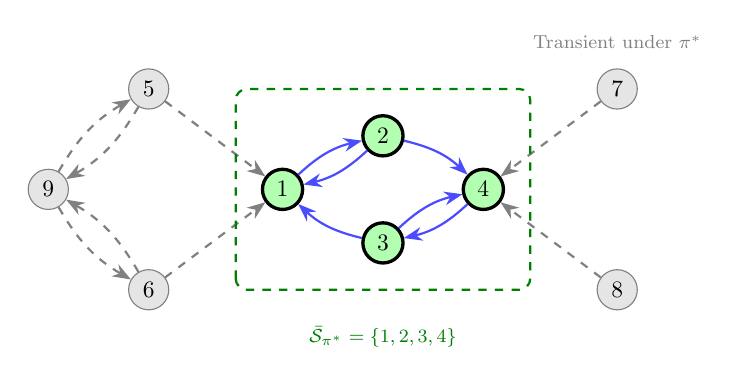
\begin{tikzpicture}[scale=0.85, transform shape]
    % Ergodic states (recurrent class) - highlighted
    \node[st, fill=green!30, line width=1.2pt] (s1) at (0, 0) {1};
    \node[st, fill=green!30, line width=1.2pt] (s2) at (1.5, 0.8) {2};
    \node[st, fill=green!30, line width=1.2pt] (s3) at (1.5, -0.8) {3};
    \node[st, fill=green!30, line width=1.2pt] (s4) at (3, 0) {4};
    
    % Transitions within ergodic set
    \draw[tr, blue!70, line width=0.8pt] (s1) to[bend left=15] (s2);
    \draw[tr, blue!70, line width=0.8pt] (s2) to[bend left=15] (s4);
    \draw[tr, blue!70, line width=0.8pt] (s4) to[bend left=15] (s3);
    \draw[tr, blue!70, line width=0.8pt] (s3) to[bend left=15] (s1);
    \draw[tr, blue!70, line width=0.8pt] (s2) to[bend left=15] (s1);
    \draw[tr, blue!70, line width=0.8pt] (s3) to[bend left=15] (s4);
    
    % Transient states - grayed out
    \node[st, fill=gray!20, draw=gray] (s5) at (-2, 1.5) {5};
    \node[st, fill=gray!20, draw=gray] (s6) at (-2, -1.5) {6};
    \node[st, fill=gray!20, draw=gray] (s7) at (5, 1.5) {7};
    \node[st, fill=gray!20, draw=gray] (s8) at (5, -1.5) {8};
    \node[st, fill=gray!20, draw=gray] (s9) at (-3.5, 0) {9};
    
    % Transient transitions (one-way into ergodic set)
    \draw[tr, gray, dashed] (s5) -- (s1);
    \draw[tr, gray, dashed] (s6) -- (s1);
    \draw[tr, gray, dashed] (s7) -- (s4);
    \draw[tr, gray, dashed] (s8) -- (s4);
    \draw[tr, gray, dashed] (s9) to[bend left=15] (s5);
    \draw[tr, gray, dashed] (s9) to[bend right=15] (s6);
    % Transitions back to s9 (creates alternative ergodic set under bad policy)
    \draw[tr, gray, dashed] (s5) to[bend left=15] (s9);
    \draw[tr, gray, dashed] (s6) to[bend right=15] (s9);
    
    % Labels
    \node[font=\footnotesize, green!50!black] at (1.5, -2.2) {$\bar{\mathcal{S}}_{\pi^*} = \{1,2,3,4\}$};
    \node[font=\footnotesize, gray] at (5, 2.2) {Transient under $\pi^*$};
    
    % Bounding box for ergodic set
    \draw[rounded corners, dashed, green!50!black, line width=0.8pt] (-0.7, -1.5) rectangle (3.7, 1.5);
\end{tikzpicture}
\end{center}

\vspace{1mm}
\begin{itemize}
    \item Even for a suboptimal policy $\pi$, once it improves sufficiently, we often have $\bar{\mathcal{S}}_{\pi} = \bar{\mathcal{S}}_{\pi^*}$.
    \item Implication: updating $V(s)$ for $s \notin \bar{\mathcal{S}}_{\pi^*}$ wastes computation---these states are never revisited.
\end{itemize}
\end{frame}



\begin{frame}{Example 2: Ergodic Set in a Growth Model}
\small
In the stochastic growth model $(k_t, z_t) \to (k_{t+1}, z_{t+1})$, the ergodic set is a small region of the state space.

\begin{center}
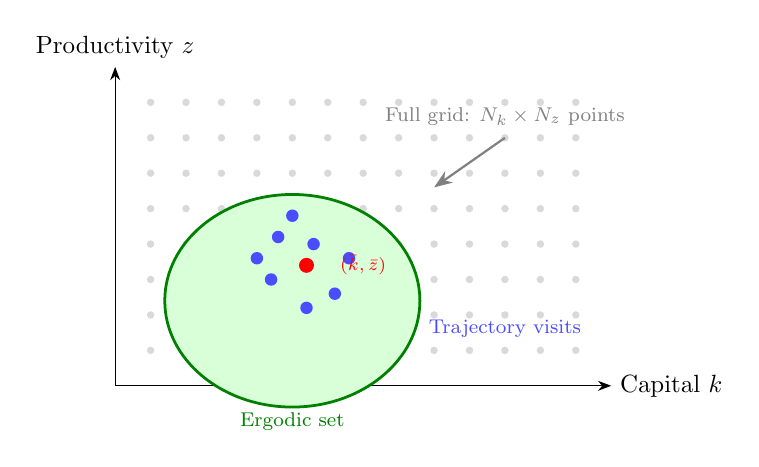
\begin{tikzpicture}[scale=0.9, transform shape]
    % Axes
    \draw[->] (0, 0) -- (7, 0) node[right] {Capital $k$};
    \draw[->] (0, 0) -- (0, 4.5) node[above] {Productivity $z$};
    
    % Full grid (light gray dots)
    \foreach \x in {0.5, 1, 1.5, 2, 2.5, 3, 3.5, 4, 4.5, 5, 5.5, 6, 6.5} {
        \foreach \y in {0.5, 1, 1.5, 2, 2.5, 3, 3.5, 4} {
            \fill[gray!30] (\x, \y) circle (1.5pt);
        }
    }
    
    % Ergodic set (ellipse region with dense points)
    \draw[fill=green!15, draw=green!50!black, line width=1pt, rounded corners] 
        (2.5, 1.2) ellipse (1.8cm and 1.5cm);
    
    % Trajectory samples within ergodic set
    \fill[blue!70] (2.2, 1.5) circle (2.5pt);
    \fill[blue!70] (2.8, 2.0) circle (2.5pt);
    \fill[blue!70] (3.1, 1.3) circle (2.5pt);
    \fill[blue!70] (2.5, 2.4) circle (2.5pt);
    \fill[blue!70] (2.0, 1.8) circle (2.5pt);
    \fill[blue!70] (3.3, 1.8) circle (2.5pt);
    \fill[blue!70] (2.7, 1.1) circle (2.5pt);
    \fill[blue!70] (2.3, 2.1) circle (2.5pt);
    
    % Steady state
    \fill[red] (2.7, 1.7) circle (3pt);
    \node[font=\scriptsize, red] at (3.5, 1.7) {$(\bar{k}, \bar{z})$};
    
    % Labels
    \node[font=\footnotesize, gray] at (5.5, 3.8) {Full grid: $N_k \times N_z$ points};
    \node[font=\footnotesize, green!50!black] at (2.5, -0.5) {Ergodic set};
    \node[font=\footnotesize, blue!70] at (5.5, 0.8) {Trajectory visits};
    
    % Annotation
    \draw[->, gray, thick] (5.5, 3.5) -- (4.5, 2.8);
\end{tikzpicture}
\end{center}

\vspace{1mm}
Judd, Maliar, Maliar \& Valero (2014): Simulated trajectories visit $<5\%$ of grid points in high-dimensional models. Updating only visited states achieves similar accuracy at a fraction of the cost.
\end{frame}




\begin{frame}{Planning vs Simulation: illustration}
\begin{center}
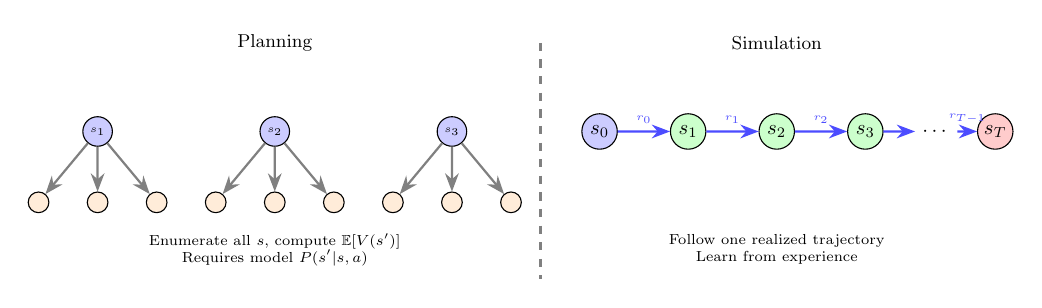
\begin{tikzpicture}[scale=0.75, transform shape]
    % LEFT: Planning - enumerate all grid points
    \node[anchor=center, font=\small] at (-4, 3) {Planning};
    
    % Grid point s_1
    \node[st, fill=blue!20, minimum size=5mm] (g1) at (-7, 1.5) {\tiny $s_1$};
    \node[st, fill=orange!15, minimum size=3.5mm] (g1a) at (-8, 0.3) {};
    \node[st, fill=orange!15, minimum size=3.5mm] (g1b) at (-7, 0.3) {};
    \node[st, fill=orange!15, minimum size=3.5mm] (g1c) at (-6, 0.3) {};
    \draw[tr, gray] (g1) -- (g1a);
    \draw[tr, gray] (g1) -- (g1b);
    \draw[tr, gray] (g1) -- (g1c);
    
    % Grid point s_2
    \node[st, fill=blue!20, minimum size=5mm] (g2) at (-4, 1.5) {\tiny $s_2$};
    \node[st, fill=orange!15, minimum size=3.5mm] (g2a) at (-5, 0.3) {};
    \node[st, fill=orange!15, minimum size=3.5mm] (g2b) at (-4, 0.3) {};
    \node[st, fill=orange!15, minimum size=3.5mm] (g2c) at (-3, 0.3) {};
    \draw[tr, gray] (g2) -- (g2a);
    \draw[tr, gray] (g2) -- (g2b);
    \draw[tr, gray] (g2) -- (g2c);
    
    % Grid point s_3
    \node[st, fill=blue!20, minimum size=5mm] (g3) at (-1, 1.5) {\tiny $s_3$};
    \node[st, fill=orange!15, minimum size=3.5mm] (g3a) at (-2, 0.3) {};
    \node[st, fill=orange!15, minimum size=3.5mm] (g3b) at (-1, 0.3) {};
    \node[st, fill=orange!15, minimum size=3.5mm] (g3c) at (-0, 0.3) {};
    \draw[tr, gray] (g3) -- (g3a);
    \draw[tr, gray] (g3) -- (g3b);
    \draw[tr, gray] (g3) -- (g3c);
    
    \node[font=\scriptsize, align=center] at (-4, -0.5) {Enumerate all $s$, compute $\mathbb{E}[V(s')]$\\Requires model $P(s'|s,a)$};
    
    % Divider
    \draw[dashed, gray, line width=0.8pt] (0.5, 3) -- (0.5, -1);
    
    % RIGHT: Simulation (Trajectory)
    \node[anchor=center, font=\small] at (4.5, 3) {Simulation};
    
    \node[st, fill=blue!20] (t0) at (1.5, 1.5) {$s_0$};
    \node[st, fill=green!20] (t1) at (3, 1.5) {$s_1$};
    \node[st, fill=green!20] (t2) at (4.5, 1.5) {$s_2$};
    \node[st, fill=green!20] (t3) at (6, 1.5) {$s_3$};
    \node (t4) at (7.2, 1.5) {$\cdots$};
    \node[st, fill=red!20] (tT) at (8.2, 1.5) {$s_T$};
    
    \draw[tr, blue!70] (t0) -- node[above, font=\tiny] {$r_0$} (t1);
    \draw[tr, blue!70] (t1) -- node[above, font=\tiny] {$r_1$} (t2);
    \draw[tr, blue!70] (t2) -- node[above, font=\tiny] {$r_2$} (t3);
    \draw[tr, blue!70] (t3) -- (t4);
    \draw[tr, blue!70] (t4) -- node[above, font=\tiny] {$r_{T-1}$} (tT);
    
    \node[font=\scriptsize, align=center] at (4.5, -0.5) {Follow one realized trajectory\\Learn from experience};
\end{tikzpicture}
\end{center}


\begin{itemize}
    \setlength\itemsep{0.5mm}
    \item Trajectory / Episode / Rollout: A sequence of states and rewards $(s_0, a_0, r_0, s_1, a_1, r_1, \ldots)$ generated by following a policy $\pi$ from initial state $s_0$ to terminal state $s_T$.
    \item The associated return is $G_0 = r_0 + \beta r_1 + \beta^2 r_2 + \cdots + \beta^T r_{T-1}$
\end{itemize}
\end{frame}




\begin{frame}{Planning: The Bellman Update}
\small
\begin{itemize}
    \item At iteration $k$, we update $V^{(k)}$ to $V^{(k+1)}$ using the Bellman equation:
        \[
            V^{(k+1)}(s) = r(s) + \beta \int V^{(k)}(s') \, P(ds'|s) = \int (\underbrace{r(s) + \beta V^{(k)}(s')}_{\text{Target}}) \, P(ds'|s)
        \]

    \item Planning computes the integral exactly (quadrature) or via MC integration with $M$ samples:
        \[
            V^{(k+1)}(s) = \frac{1}{M} \sum_{m=1}^{M} \big[ r(s) + \beta V^{(k)}(s'_m) \big] = \frac{1}{M} \sum_{m=1}^{M} \text{Target}^{(k)}_m 
        \]
    \item Simulation-based: sample size $M = 1$ and incremental update weighted by $\alpha_k$ (learning rate):
        \begin{align*}
            V^{(k+1)}(s) &= V^{(k)}(s) + \alpha_k \big[ \underbrace{r + \beta V^{(k)}(s') - V^{(k)}(s)}_{\text{Bellman residual $\delta_k$}} \big] \\
            &= (1 - \alpha_k) \cdot \underbrace{V^{(k)}(s)}_{\text{old estimate}} + \alpha_k \cdot \underbrace{\big[ r(s) + \beta V^{(k)}(s') \big]}_{\text{Target}}
        \end{align*}
\end{itemize}
\end{frame}

\begin{frame}{Convergence: Simulation $\to$ Planning}
    \small
    \begin{itemize}
        \item Suppose state $s$ has been visited $n(s)$ times.  
              On the $n(s)$-th visit, choose $\alpha_{n(s)} = \frac{1}{n(s)}$, which satisfies the Robbins--Monro conditions: $\sum_k \alpha_k = \infty$ and $\sum_k \alpha_k^2 < \infty$.
    
        \item The simulation update on the $n(s)$-th visit becomes
              \[
                  V^{(k+1)}(s) = V^{(k)}(s) + \frac{1}{n(s)} \big[ \underbrace{r(s) + \beta V^{(k)}(s')}_{\text{Target}_{n(s)}} - V^{(k)}(s) \big]
                  = \frac{1}{n(s)} \, \text{Target}_{n(s)} + \frac{n(s)-1}{n(s)}\,V^{(k)}(s)
              \]
    
        \item Unrolling: substitute $V^{(k)}(s) = \frac{1}{n(s)-1}\text{Target}_{n(s)-1} + \frac{n(s)-2}{n(s)-1}V^{(k-1)}(s)$, and repeat:
              \begin{align*}
                  V^{(k+1)}(s) &= \frac{1}{n(s)} \, \text{Target}_{n(s)} + \frac{n(s)-1}{n(s)} \cdot \frac{1}{n(s)-1} \, \text{Target}_{n(s)-1} + \cdots \\
                  &= \frac{1}{n(s)} \, \text{Target}_{n(s)} + \frac{1}{n(s)} \, \text{Target}_{n(s)-1} + \cdots + \frac{1}{n(s)} \, \text{Target}_1 \\
                  &= \frac{1}{n(s)} \sum_{i=1}^{n(s)} \text{Target}_i
              \end{align*}


    \end{itemize}
    \end{frame}



\begin{frame}{Temporal Difference (TD) Learning: Formal Introduction}
\small
\begin{itemize}
    \item The simulation-based update we derived uses the estimated value $V(s_{t+1})$ to update $V(s_t)$. This is called \emph{bootstrapping}: updating an estimate based on another estimate. (This differs from the bootstrap in statistics, which is resampling from data to estimate uncertainty.)
    \item Simulation-based methods with bootstrapping are called Temporal Difference (TD) learning:
    \[
        V(s_t) \;\leftarrow\; V(s_t) + \alpha \cdot \big( r_t + \beta V(s_{t+1}) - V(s_t) \big), \quad \text{where } s_t \sim \bar{\mathcal{S}}_{\pi}
    \]
    \item The name ``Temporal Difference'' refers to the difference between value estimates at two successive time points: $V(s_{t+1})$ vs $V(s_t)$.
    \item The Bellman residual $\delta_t = r_t + \beta V(s_{t+1}) - V(s_t)$ is also called the TD error.
    \item This specific update rule is called TD(0). The ``0'' indicates that we bootstrap immediately after observing just one reward $r_t$, using zero additional steps before estimating the remaining value via $V(s_{t+1})$.
\end{itemize}   
\end{frame}





\begin{frame}{TD(0) Algorithm for Policy Evaluation}
\small
\begin{itemize}
    \setlength\itemsep{1.5mm}
    \item Step 0 (inputs): Policy $\pi$ to evaluate; discount $\beta \in (0,1)$; learning rate schedule $\{\alpha_k\}$; number of episodes $K$; initial state distribution $\mu_0$.
    
    \item Step 1 (initialize): For all states $s \in \mathcal{S}$, set $V^{(0)}(s) \leftarrow 0$ (or arbitrary values).
    
    \item Step 2 (episode loop): For episode $k = 1, 2, \ldots, K$:
    \begin{itemize}
        \setlength\itemsep{1mm}
        \item Sample initial state $s_0 \sim \mu_0$.
        \item For $t = 0, 1, 2, \ldots$ until terminal state:
        \begin{enumerate}
            \item Take action $a_t = \pi(s_t)$, observe reward $r_t$ and next state $s_{t+1}$.
            \item Compute TD error: $\delta_t = r_t + \beta \, V(s_{t+1}) - V(s_t)$.
            \item Update: $V(s_t) \leftarrow V(s_t) + \alpha_k \cdot \delta_t$.
        \end{enumerate}
    \end{itemize}
    
    \item Step 3 (output): Value function estimate $V \approx V^\pi$.

\end{itemize}
\end{frame}


\begin{frame}{The Exploration Problem: Ergodic Set Depends on $\pi$}
    \small
    \begin{itemize}
        \item The ergodic set of states visited under a policy,
        \[
            \bar{\mathcal{S}}_\pi = \{s : \Pr_\pi(s_t = s \text{ for some } t) > 0\},
        \]
        depends on the policy $\pi$ itself.
    
        \item During learning, the policy evolves:
        \[
            \pi^{(0)} \to \pi^{(1)} \to \pi^{(2)} \to \cdots \to \pi^*.
        \]
    
        \item This creates a fundamental difficulty:
        \begin{itemize}
            \item Accurate estimation of $V(s)$ requires many visits to state $s$.
            \item But the states we visit depend on the current policy $\pi^{(k)}$.
            \item A poor early policy may prevent us from ever reaching states that matter under $\pi^*$.
        \end{itemize}
    
        \item Consequences of poor initialization:
        \begin{itemize}
            \setlength\itemsep{1.5mm}
            \item $\bar{\mathcal{S}}_{\pi^{(0)}}$ may omit states in $\bar{\mathcal{S}}_{\pi^*}$.
            \item For such states, $V(s)$ is never updated.
            \item Policy improvement cannot discover these states, and learning becomes trapped in a suboptimal region.
        \end{itemize}
    
        \item This is the exploration–exploitation problem: we must allow for exploration of unfamiliar states while still improving the policy using available information.
    \end{itemize}
    \end{frame}



\begin{frame}{Example: How Poor Initialization Causes Suboptimal Convergence}
\small
Same 9-state MDP, but now consider a poorly initialized policy $\pi^{(0)}$ that gets stuck in $\{5, 6, 9\}$.

\begin{center}
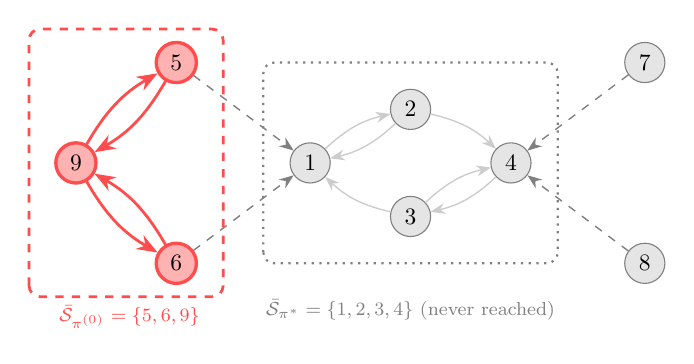
\begin{tikzpicture}[scale=0.85, transform shape]
    % Optimal ergodic states - grayed out (not visited under bad policy)
    \node[st, fill=gray!20, draw=gray] (s1) at (0, 0) {1};
    \node[st, fill=gray!20, draw=gray] (s2) at (1.5, 0.8) {2};
    \node[st, fill=gray!20, draw=gray] (s3) at (1.5, -0.8) {3};
    \node[st, fill=gray!20, draw=gray] (s4) at (3, 0) {4};
    
    % Transitions within optimal ergodic set (grayed out - same as Figure 1)
    \draw[tr, gray!40, line width=0.5pt] (s1) to[bend left=15] (s2);
    \draw[tr, gray!40, line width=0.5pt] (s2) to[bend left=15] (s4);
    \draw[tr, gray!40, line width=0.5pt] (s4) to[bend left=15] (s3);
    \draw[tr, gray!40, line width=0.5pt] (s3) to[bend left=15] (s1);
    \draw[tr, gray!40, line width=0.5pt] (s2) to[bend left=15] (s1);
    \draw[tr, gray!40, line width=0.5pt] (s3) to[bend left=15] (s4);
    
    % Bad policy ergodic states - highlighted in red
    \node[st, fill=red!30, line width=1.2pt, draw=red!70] (s5) at (-2, 1.5) {5};
    \node[st, fill=red!30, line width=1.2pt, draw=red!70] (s6) at (-2, -1.5) {6};
    \node[st, fill=red!30, line width=1.2pt, draw=red!70] (s9) at (-3.5, 0) {9};
    
    % Other transient states
    \node[st, fill=gray!20, draw=gray] (s7) at (5, 1.5) {7};
    \node[st, fill=gray!20, draw=gray] (s8) at (5, -1.5) {8};
    
    % Transitions in bad policy ergodic set (active)
    \draw[tr, red!70, line width=1pt] (s9) to[bend left=15] (s5);
    \draw[tr, red!70, line width=1pt] (s5) to[bend left=15] (s9);
    \draw[tr, red!70, line width=1pt] (s9) to[bend right=15] (s6);
    \draw[tr, red!70, line width=1pt] (s6) to[bend right=15] (s9);
    
    % Unused transitions (to optimal set) - same as Figure 1
    \draw[tr, gray, dashed, line width=0.5pt] (s5) -- (s1);
    \draw[tr, gray, dashed, line width=0.5pt] (s6) -- (s1);
    \draw[tr, gray, dashed, line width=0.5pt] (s7) -- (s4);
    \draw[tr, gray, dashed, line width=0.5pt] (s8) -- (s4);
    
    % Labels
    \node[font=\footnotesize, red!70] at (-2.7, -2.3) {$\bar{\mathcal{S}}_{\pi^{(0)}} = \{5,6,9\}$};
    \node[font=\footnotesize, gray] at (1.5, -2.2) {$\bar{\mathcal{S}}_{\pi^*} = \{1,2,3,4\}$ (never reached)};
    
    % Bounding box for bad ergodic set
    \draw[rounded corners, dashed, red!70, line width=1pt] (-4.2, -2) rectangle (-1.3, 2);
    
    % Bounding box for optimal ergodic set (grayed)
    \draw[rounded corners, dotted, gray, line width=0.8pt] (-0.7, -1.5) rectangle (3.7, 1.5);
\end{tikzpicture}
\end{center}

\vspace{1mm}
\begin{itemize}
    \setlength\itemsep{0.5mm}
    \item Policy $\pi^{(0)}$ cycles within $\{5, 6, 9\}$ --- never transitions to state 1.
    \item $V(s)$ for $s \in \{1,2,3,4\}$ never gets updated $\Rightarrow$ cannot discover higher rewards there.
    \item Learning is stuck: $\bar{\mathcal{S}}_{\pi^{(0)}} \cap \bar{\mathcal{S}}_{\pi^*} = \emptyset$.
\end{itemize}
\end{frame}






\begin{frame}{Solutions to the Exploration Problem}
\small
\begin{itemize}
    \setlength\itemsep{1.5mm}
    \item $\varepsilon$-greedy policy:
    \begin{itemize}
        \item With probability $1-\varepsilon$: follow the current best policy
        \item With probability $\varepsilon$: take a random action
        \item Ensures all state-action pairs have positive visitation probability
    \end{itemize}
    
    \item Optimistic initialization:
    \begin{itemize}
        \item Initialize $V(s)$ to high values (optimistic about unexplored states)
        \item Agent is ``curious'' --- explores until reality disappoints the optimism
    \end{itemize}
    
    \item Exploring starts:
    \begin{itemize}
        \item Begin episodes from randomly chosen states
        \item Guarantees coverage of the full state space over time
    \end{itemize}
    
    \item Key insight: Exploration is the price we pay for not knowing the model. Planning (with known $P$) can evaluate all states without visiting them; simulation cannot.
\end{itemize}
\end{frame}



\begin{frame}{TD Learning: Advantages and Disadvantages}
    \small
    \begin{itemize}
        \item Advantages:
        \setlength\itemsep{1.5mm}
        \begin{itemize}
            \item Model-free: No need to know the transition probabilities $P$.
            \item Scalable: DP must iterate over all states each sweep; TD only updates visited states, making it feasible for large or continuous state spaces.
            \item Computationally cheaper: No integration required
        \end{itemize}
        \item Disadvantages :
        \setlength\itemsep{1.5mm}
        \begin{itemize}
            \item Noisy updates: using one sample $s'$ instead of integrating over all possible $s'$ introduces variance.
            \item Exploration required: Only visited states get updated. 
            \item Slower convergence: Stochastic approximation converges at $O(1/\sqrt{n})$; DP with known model converges geometrically.
            \item Learning rate tuning: Performance depends on $\alpha$. DP has no such hyperparameter.
        \end{itemize}
    \end{itemize}
    \end{frame}
    
    


%===================================================
% THE SPECTRUM OF METHODS: FROM TD(0) TO MC
%===================================================

\begin{frame}{Generalizing TD(0): The $n$-Step Return}
\small
\begin{itemize}
    \item Recall TD(0) bootstraps after observing just one reward:
    \[
        G_t^{(1)} = r_t + \beta V(s_{t+1})
    \]
    \item What if we wait longer? Observe $n$ actual rewards before bootstrapping:
    \[
        G_t^{(n)} = r_t + \beta r_{t+1} + \beta^2 r_{t+2} + \cdots + \beta^{n-1} r_{t+n-1} + \beta^n V(s_{t+n})
    \]
    \item The $n$-step return uses $n$ realized rewards and bootstraps from $V(s_{t+n})$.
    \item Examples:
    \begin{itemize}
        \item $n=1$ (TD(0)): $G_t^{(1)} = r_t + \beta V(s_{t+1})$
        \item $n=2$: $G_t^{(2)} = r_t + \beta r_{t+1} + \beta^2 V(s_{t+2})$
        \item $n=3$: $G_t^{(3)} = r_t + \beta r_{t+1} + \beta^2 r_{t+2} + \beta^3 V(s_{t+3})$
    \end{itemize}
    \item As $n$ increases, we rely more on actual rewards and less on the estimated value.
\end{itemize}
\end{frame}

\begin{frame}{The Two Extremes: TD(0) and Monte Carlo}
\small
\begin{itemize}
    \item TD(0) ($n=1$): Bootstrap immediately after one reward.
    \[
        G_t^{(1)} = \underbrace{r_t}_{\text{1 actual reward}} + \underbrace{\beta V(s_{t+1})}_{\text{bootstrap}}
    \]
    \begin{itemize}
        \item[\ding{51}] Low variance: only one random transition affects the target.
        \item[\ding{55}] Biased: relies on current (imperfect) estimate $V(s_{t+1})$.
    \end{itemize}
    
    \item Monte Carlo ($n = T-t$, i.e., wait until episode ends): No bootstrapping at all.
    \[
        G_t^{(\infty)} = \underbrace{r_t + \beta r_{t+1} + \beta^2 r_{t+2} + \cdots + \beta^{T-t} r_T}_{\text{all actual rewards, no bootstrap}}
    \]
    \begin{itemize}
        \item[\ding{51}] Unbiased: $G_t^{(\infty)}$ is a true sample of $V(s_t)$.
        \item[\ding{55}] High variance: depends on many random transitions.
        \item[\ding{55}] Must wait for episode to end before updating.
    \end{itemize}
\end{itemize}
\end{frame}


\begin{frame}{Visualizing the Spectrum: Backup Diagrams}
\begin{center}
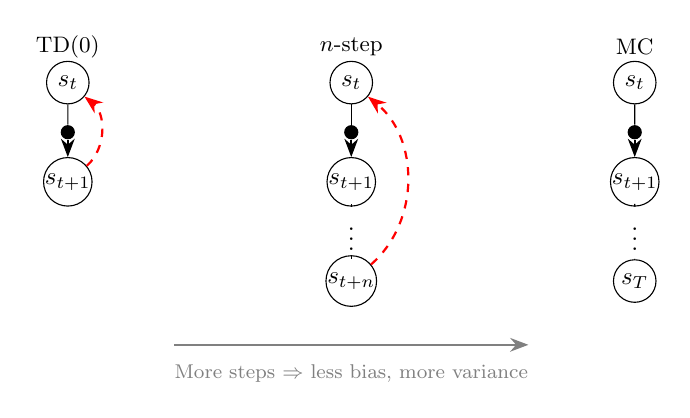
\begin{tikzpicture}[scale=0.9, transform shape]
    % TD(0) Backup
    \node[anchor=center] at (-4, 3) {\small TD(0)};
    \node[st] (td0) at (-4, 2.5) {$s_t$};
    \node[action] (tda0) at (-4, 1.8) {};
    \node[st] (td1) at (-4, 1.1) {$s_{t+1}$};
    
    \draw (td0) -- (tda0);
    \draw[tr] (tda0) -- (td1);
    \draw[dashed, red, thick, ->] (td1) to[bend right=50] node[left, font=\tiny, color=red] {} (td0);

    % n-step Backup
    \node[anchor=center] at (0, 3) {\small $n$-step};
    \node[st] (ns0) at (0, 2.5) {$s_t$};
    \node[action] (nsa0) at (0, 1.8) {};
    \node[st] (ns1) at (0, 1.1) {$s_{t+1}$};
    \node (ns2) at (0, 0.4) {$\vdots$};
    \node[st] (nsn) at (0, -0.3) {$s_{t+n}$};
    
    \draw (ns0) -- (nsa0);
    \draw[tr] (nsa0) -- (ns1);
    \draw (ns1) -- (ns2);
    \draw (ns2) -- (nsn);
    \draw[dashed, red, thick, ->] (nsn) to[bend right=50] node[left, font=\tiny, color=red] {} (ns0);

    % MC Backup
    \node[anchor=center] at (4, 3) {\small MC};
    \node[st] (mc0) at (4, 2.5) {$s_t$};
    \node[action] (a0) at (4, 1.8) {};
    \node[st] (mc1) at (4, 1.1) {$s_{t+1}$};
    \node (mc2) at (4, 0.4) {$\vdots$};
    \node[st] (mcT) at (4, -0.3) {$s_T$};
    
    \draw (mc0) -- (a0);
    \draw[tr] (a0) -- (mc1);
    \draw (mc1) -- (mc2);
    \draw (mc2) -- (mcT);
    
    % Arrows for spectrum
    \draw[->, thick, gray] (-2.5, -1.2) -- (2.5, -1.2);
    \node[font=\footnotesize, gray] at (0, -1.6) {More steps $\Rightarrow$ less bias, more variance};
\end{tikzpicture}
\end{center}
\begin{itemize}
    \item TD(0): Bootstrap after 1 step (red arrow shows bootstrap).
    \item $n$-step: Bootstrap after $n$ steps.
    \item MC: No bootstrap---use full trajectory to terminal state $s_T$.
\end{itemize}
\end{frame}



\begin{frame}{TD(0) vs MC: The Bias-Variance Trade-off}
    \small
    \begin{itemize}
        \item TD(0) is based and MC is unbias:
            \begin{itemize}
                \item TD(0): $r_t + \beta V(s_{t+1})$ is based on the estimated value $V(s_{t+1})$, which is our current guess---not the true value. We are ``updating a guess towards another guess.''
                \item MC: base on the actual realized rewards, which is a random variable whose expectation equals the true $V(s_t)$.
            \end{itemize}
        \item TD(0) has lower variance than MC:
            \begin{itemize}
                \item TD(0): depends on only one random transition $(s_t, r_t, s_{t+1})$.
                \item MC: accumulates randomness from all transitions in the episode: $(s_t, r_t, s_{t+1}), (s_{t+1}, r_{t+1}, s_{t+2}), \ldots$
            \end{itemize}
        \item The $n$-step return interpolates: larger $n$ means less bias but more variance.
    \end{itemize}
    \end{frame}


\begin{frame}{TD($\lambda$): A Weighted Blend of All $n$-Step Returns}
\small
\begin{itemize}
    \item Instead of choosing a single $n$, why not combine all $n$-step returns?
    \item The $\lambda$-return takes a weighted average with geometrically decaying weights:
    \[
        G_t^\lambda = (1-\lambda) \sum_{n=1}^{T-t-1} \lambda^{n-1} G_t^{(n)} + \lambda^{T-t-1} G_t^{(T-t)}
    \]
    \item The parameter $\lambda \in [0,1]$ controls the decay:
    \begin{itemize}
        \item Weight on $G_t^{(1)}$: $(1-\lambda)$
        \item Weight on $G_t^{(2)}$: $(1-\lambda)\lambda$
        \item Weight on $G_t^{(3)}$: $(1-\lambda)\lambda^2$
        \item $\vdots$
    \end{itemize}
    \item Special cases:
    \begin{itemize}
        \item $\lambda = 0$: All weight on $G_t^{(1)}$ $\Rightarrow$ TD(0).
        \item $\lambda = 1$: All weight on $G_t^{(\infty)}$ $\Rightarrow$ Monte Carlo.
    \end{itemize}
\end{itemize}
\end{frame}

%===================================================
% NUMERICAL COMPARISON
%===================================================

\begin{frame}{Numerical Experiment: VFI vs TD Policy Evaluation}
\small
Setup: Evaluate the \emph{same} optimal policy $\pi^*$ (solved by VFI) using different methods.

\vspace{2mm}
\begin{itemize}
    \setlength\itemsep{1.5mm}
    \item Model: Consumption-saving with discrete assets and income shocks.
    \item Ground truth: $V^{\text{VFI}}$ from exact dynamic programming.
    \item TD evaluation: Run TD($\lambda$) for $\lambda \in \{0, 0.5, 0.9, 1.0\}$.
    \item Repeat each TD method 5 times with different random seeds.
\end{itemize}

\vspace{2mm}
Metrics:
\begin{itemize}
    \setlength\itemsep{1mm}
    \item MSE: $\frac{1}{|\mathcal{S}|} \sum_s (V^{\text{TD}}(s) - V^{\text{VFI}}(s))^2$ (bias + variance)
    \item Variance: $\frac{1}{|\mathcal{S}|} \sum_s \text{Var}[V^{\text{TD}}(s)]$ across runs
\end{itemize}

\vspace{2mm}
Key insight: All methods evaluate the \emph{same} policy---differences are purely due to estimation method.
\end{frame}

\begin{frame}[fragile]{Code: Comparing VFI and TD($\lambda$)}
\small
\begin{verbatim}
from model import create_default_model
from algos import compare_vfi_td

model = create_default_model()
results = compare_vfi_td(
    model,
    lambdas=[0.0, 0.5, 0.9, 1.0],
    n_runs=5,
    n_episodes=5000,
    alpha=0.5
)

# Results contain:
# - V_vfi: exact value function from VFI
# - td_results[lambda]: V_mean, V_std, mse, avg_variance
\end{verbatim}

See \texttt{Lab\_8\_Simulation\_Based\_Learning/} for full implementation.
\end{frame}

\begin{frame}{Expected Results: Bias-Variance Trade-off}
\small
\begin{center}
\begin{tabular}{l|ccc}
\toprule
Method & MSE vs VFI & Avg Variance & Interpretation \\
\midrule
TD(0), $\lambda=0$ & Medium & Low & High bias, low variance \\
TD(0.5) & Lower & Medium & Balanced \\
TD(0.9) & Lower & Higher & Less bias, more variance \\
MC, $\lambda=1$ & Lowest bias & Highest & Unbiased but noisy \\
\bottomrule
\end{tabular}
\end{center}

\vspace{3mm}
Observations:
\begin{itemize}
    \setlength\itemsep{1.5mm}
    \item TD(0) converges fast but may have residual bias (depends on $\alpha$ schedule).
    \item MC is unbiased in the limit but requires many episodes to reduce variance.
    \item Intermediate $\lambda$ (e.g., 0.9) often achieves the best MSE in practice.
    \item All TD methods are slower than VFI when the model is known---but TD works without knowing $P$.
\end{itemize}
\end{frame}

\end{document}